%**
%*  @file  source_tree.tex
%*  @brief  DIET Programmer' guide - chapter two
%*  @author  Philippe Combes (Philippe.Combes@ens-lyon.fr)
%*  @section Licence 
%*    |LICENSE|


There are two main source directories, \textsf{include} and \textsf{src}, and
the \textsf{doc} directory.


\section{\textsf{doc}}
\label{s:doc}

This directory contains documentations that are to be maintained up-to-date,
even in CVS, (\emph{ie} \textbf{not only for releases !}):

  \begin{itemize}
  \item \textsf{doc/UsersManual} contains the \textit{User's Manual}. 
     Its output file is \texttt{DIET\_UsersManual.ps}, which is intalled in
     \texttt{$<$install\_dir$>$/doc}.
  \item \textsf{doc/ProgrammersGuide} holds the \textit{Programmer's Guide}.
     Its output file is \texttt{DIET\_ProgrammersGuide.ps}, which is intalled
     in \texttt{$<$install\_dir$>$/doc}, \textbf{if} DIET has been configured
     in maintainer mode.
  \item \textsf{doc/Tutorial} holds a tutorial, which is only available
     in the CVS version, since the distribution of this tutorial is apart
     from the distribution of the source code.
  \item \textsf{doc/ExternalExample} contains a minimal set of files
     that enable to illustate how a DIET user can compile and link
     against an installation of DIET.
     This can be done both with \verb+make+ and \verb+cmake+.
     Note that the purpose of this directory is not to demonstrate
     DIET features.
     Nevertheless, the very simple DIET client/server example is effective
     DIET code.
  \end{itemize}

  The compilation of this documentation may require too recent versions of
  \LaTeX and of various converters for the figures.
  This is why, the output \textsf{.ps} files are included in the distributions.

  \section{\textsf{include}}
  \label{s:include}

  This directory contains all the files necessary for the DIET user to program his
  application. Almost all these files are headers which are copied into the
  \textsf{$<$install\_dir$>$/include} directory, because they describe the
  complete API of DIET, for the client side as well as for the server side.

  Nevertheless, there is also a \texttt{Makefile.inc.in} which will be configured
  into a \texttt{Makefile.inc}.
  The latter is to be included by the \texttt{Makefile} of the
  DIET user, to set all options and variables necessary for compiling and
  linking with the DIET libraries.
  It may be noticed that some variables are affected with
  \texttt{?=} ; it is because the \texttt{Makefile.inc} is also included by the
  DIET examples, which need to define a different prefix as long as the
  \texttt{make install} has not been invoked.



  \subsubsection{\tt DIET\_data.h}

  The first file to be included. It describes all types and data structures (and
      the associated functions and macros) that are common to the interfaces of the
  client and the server: \verb+diet_arg_t+, \verb+diet_profile_t+, \verb+*_set+
  and \verb+*_get+ functions, \verb+diet_free_data+, etc.

  Please note that the \verb+*_get+ functions are actually macros, which allows
  the user not to care about the type of the data. But the compilation of a
  program that uses such macros could trigger a warning about ``strict aliasing''.
  This is the case for the distributed examples, when compiled with
\textsf{gcc-3.3} or later (see section \ref{s:examples})


  \subsubsection{{\tt DIET\_client.h} and {\tt DIET\_grpc.h}}

  The specific part of the client interface is described in these two files.
  \textsf{DIET\_client.h} includes \textsf{DIET\_grpc.h}, which includes itself
  \textsf{DIET\_data.h}.
  The first file is the DIET specific API, adpated and optimized for the data
  structures of DIET. The second file consists of the GridRPC API, even if some of
  the functions are not fully implemented (for more details, please read the
      numerous comments of the file itself).


  \subsubsection{\tt DIET\_server.h}

  This file contains the specific part of the server API.
  It offers functions and macros to manipulate the description of the service
  profiles (\verb+diet_profile_desc_t+), and store them into the service table of
  the server (\verb+diet_*service_table*+). Everything that concerns the problem
  profiles (how to extract their arguments, set their OUT arguments, etc.) is
  described in \texttt{DIET\_data.h}.


  There is also the complete API to the \texttt{diet\_convertor\_t} structures.
  Their usage are (or should be) explained in the \textit{User's Manual}, and the
  way they are applied is fully documented in section \ref{s:CORBA}, since the
  conversions are performed by functions of the file \texttt{marshalling.cc}.

  \subsubsection{\tt DIET\_mutex.h}

  This is intented to be a portable API to the various thread libraries, a bit
  like the \textsf{omnithread} library. But the \textsf{omnithread} library is a
  portable API for all thread systems (pthreads for Linux, but also the official
      thread libraries of other platforms), and {\tt DIET\_mutex.h} should only unify
  the APIs of different ORBs, since they all offer a portable thread library.
  Thus, as well as an application using \textsf{omniORB} should use the
  \textsf{omnithread} library if it has to deal with threads, an application using
  DIET will have to use the DIET thread library.

  It is not documented yet in the \textit{User's Manual} because it is really not
  ready to be distributed. Currently it deals only with mutexes, and waits for a
  complete development...



  \section{\textsf{src/agent}}
  \label{s:agent}

  \subsection{The hierarchy of agents}

  This section deals with the inheritance of the C++ agent classes and the way an
  agent refers to its children. The inheritance hierarchy of the CORBA objects
  will be treated in section \ref{s:IDL}.
  \\

  The hierarchy of the C++ classes that implement the CORBA interfaces is mapped
  onto the hierarchy of theses interfaces, \emph{i.e.} \textsf{LocalAgentImpl} and
  \textsf{MasterAgentImpl} both inherit from \textsf{AgentImpl}. Thus, Most of the
  public function members of each class are implementations of IDL methods.

  In \textsf{AgentImpl}, \texttt{getName} is especially added for the data
  persistency architecture.

  In all classes, it has been added a \texttt{run} method that makes the
  \texttt{main} function (in \texttt{dietAgent.cc}) launch the agent. This method
  has two parts: the generic part is declared and implemented in the
  \textsf{AgentImpl} class, and the parts specific to the LA or the MA are
  declared in these classes. As these declarations overwrite the \texttt{run}
  method of \textsf{AgentImpl}, their implementations call explicitly the parent
  method.

  The protected part of the \textsf{AgentImpl} is inherited by both the
  \textsf{LocalAgentImpl} and \textsf{MasterAgentImpl}, and it groups the common
  members (the \textsf{ServiceTable}, the lists of children and requests, etc.) as
  well as the common parts of the code: the way to forward a request, to aggregate
  the responses, and some methods useful in all these jobs.
  \\

  The architecture of agents is handled with a pointer to the parent
  (\verb+Agent_var parent;+) in \textsf{LocalAgentImpl}, and two vectors of children
  in \textsf{AgentImpl}, one for LAs and one for SeDs. These vectors of children are
  actually \textsf{ts\_vectors} of instances of \textsf{NodeDescription}. The
  latter has to store information such as the hostname, the child ID (since
      children are referred to with their indexes in the vectors) but above all the
  CORBA reference of the child (an \textsf{LA\_var} or an \textsf{SeD\_var}). That
  is why it has to be a template.


  \subsection{The requests}

  The requests are managed through a class that stores all informations
  about the requests, such as their ID, the responses returned by the SeD and LA
  and the scheduler to use for the request.

  A mechanism have been developed to manage the waiting of all the responses
  returned by the SeD and LA. The \texttt{waitResponses()} methods will block the
  current thread until a defined number of call of the \texttt{addResponse()}
  method have been made. Look at the doxygen documentation for more information.


  \subsection{The schedulers}

  When all the children of an agent have sent back their responses, the agent must
  aggregate and sort them into the one single response it will sent to its parent.
  This aggregation/sort is performed by the scheduler classes.

  The starting point of the development of these scheduler classes was a
  combination of two ideas:
  \begin{itemize}
  \item Some servers would never have FAST fully installed. Either because FAST or
  NWS does not support the hardware architecture, or because the services
  offered cannot be described in the FAST ``language'' accurately enough for a
  valid bench campaign or estimation, etc. The information that the servers can
  give to the scheduler are very heterogeneous, and the old DIET scheduler was
  dealing with only the FAST estimations.\\
  An other tool has been implemented, called CoRI, and will be used to get by 
  default the information and to get other types of information (total memory,...).
  At the moment it is not compiled/called by default. This will be change when
  it is matured. See section \ref{subsection:performance} for more information.
  \item For research aspects on the platform, it would be very interesting to
  have pluggable schedulers. As the old scheduler was integrated to the agent,
  the first step towards pluggable schedulers was building classes responsible
  for the scheduling.\\
\fixme{plugin is made by alan su!}
  \end{itemize}

  The heterogeneity of the information given by the servers is due to the fact
  that all servers cannot provide the same level of accuracy about the evaluation
  of a request. We have thought of 4 different levels of accuracy, and one
  \textsf{Scheduler} class deals with one and only one level.
  \begin{enumerate}
  \item No information at all: such servers are not sorted but placed randomly.
  \item Last solve time: such server are sorted according to the last solve time.
  \item Hardware information (disk space, RAM, CPU speed, etc.): not managed yet.
  \item Dynamic information (CPU load, free memory, given by NWS): such servers
  are sorted according to their weight, which is a polynom of these
  characteristics, including the data transfer time if available.
  \item Estimation of the computation time (performed by FAST): such servers
  are sorted according to the computation time estimated plus the data transfer
  time estimated.
  \end{enumerate}

  Actually, there are only four schedulers implemented, because nothing has been
  done yet for the servers to get static information (level 3).\\
  Actually, with the compiling option --enable-cori only scheduling with round
  robin (last solve time - level 2) and random scheduling (level 1) is possible.
  There are multiple reasons why no other scheduling is possible:
\begin{enumerate}
  \item The NWS scheduling is bogus: the weight for the memory is too
  heavy in comparison with the free CPU. Fixing is not so easy, so
  we deciding to test with several plugin schedulers their
  performance, before implementing a default scheduling.
  \item To avoid an increasing complexity of the context.
  \item To avoid a single server equipped with FAST will always be chosen by
  the agent.
  \item The plugin scheduler can be used now with all power, it will
  be possible to define a scheduler for each server. It is very easy to recreate the old 
fast scheduling by the plug-in.
  \end{enumerate}


  Once the schedulers have sorted every group of servers, the most difficult is
  still to do. How to combine the various information of the servers to get a
  whole sorted list ? Which parameters should we give priority to ? This is the
  role of the \textsf{GlobalScheduler} classes. They are schedulers of the
  schedulers. A \textsf{GlobalScheduler} has got a sorted list of schedulers
  (\texttt{SchedList schedulers}) to apply onto the lists of servers. This
  presents the drawback that the agent sorts by category of information before
  sorting the servers inner each category: it is not possible to mix the various
  categories yet. But it would be easy to implement schedulers that take into
  account all type of information, computing a weight as for NWS information. It
  is just not done, because our goal was to build a frame for developping new
  schedulers, and not to test various policies.

  The only \textsf{GlobalScheduler} available so far (\textsf{StdGS}) calls first
  the \textsf{FASTScheduler} onto the list, putting ahead the servers that could
  estimate the request, then the \textsf{NWSScheduler} (for NWS information), then
  the \textsf{RRScheduler} and finally the \textsf{RandScheduler} that add the
  servers randomly into the list.
  \\

  Several drawbacks can be noticed about such a structure of schedulers:
  \begin{itemize}
  \item It is not possible to mix the various categories of servers.
  \item The schedulers are not pluggable at all.
  \item A global scheduler must be associated to each request, so that every
  agent, at every level, will schedule it the same way. But if we let the
  servers decide, they will choose different schedulers ; so only the MA can
  choose it, and as soon as the request arrives from the client ! Then it
  forwards the scheduler (its serialzed form actually) with the request, before
  it gets any information about the servers.
  \item The classes \textsf{GlobalScheduler} and \textsf{Scheduler} are actually
  virtual (because of their respective \texttt{sort} method). Thus, they
  constitue an interface that every new scheduler (global or not) should
  implements, and some maintainers may find this interface a bit too rigid, but
  it is the only way I found to get the scheduler out of the agent.
  \end{itemize}

  Despite these drawbacks, it is now much easier to change the scheduler used in
  the agent. But there is still a lot to do to reach the pluggable schedulers, if
  ever it is possible.

  \subsection{Performance prediction}\label{subsection:performance}
  CoRI is now implemented to get more information about the SeD.
  It is called by the server's side and (in FAST mode) on the agent's side. 
  CoRI is a simple super layer that manages multiple sub modules. One module
  is Cori-Easy; another is FAST.

  \subsubsection{Using Cori}
  The programmer of DIET services will use the
  interface proposed in the SeD interface file, \textsf{DIET\_server.h}
  Using CoRI as programmer DIET, use directly the
  \textsf{CORIMgr.hh}
  The starting phase of cori can be described as follow:
   \begin{itemize}
  \item All desired collectors will be add by \texttt{add} 
  \item Launch the \texttt{startCollectors} to initialising some collectors
    (i.e FAST) on startup of the server
  \item using the \textsf{call\_cori\_mgr} function on 
    demand to get a value in the estVector.
  \end{itemize}
  
  Additional to the tags that the programmer of DIET
  service can use, the DIET programmer can use 
  the tag EST\_COMMTIME for FAST. It is agent side only. 

  \subsubsection{CoRI-Easy}
  Cori-Easy is based on basic system calls. There are different
   levels to obtain this information: 
  The best way is the most portable way: The standard C library. For examples the
  functions \texttt{get\_Write\_Speed} and \texttt{get\_Read\_Speed} are written in pure C.
  OmniORB is used by DIET and it needs the GNU Library C standard, 
  so this library is the next level.
  The third level is the POSIX standard. Remark: even if Red Hat 
  say they follow the POSIX standard, this doesn't mean that you have to include the same file
  to get the function of the POSIX standard (for example \texttt{getPID()}). 
  It means you can never be sure to have the function!
  The fourth level is the distribution of the operating system, 
  but even here you have to take care(new version-old version conflicts). 
  System calls are very fragile, point of view accessibility 
  (they are not always present or you have to be root to execute them)
  , point of view functionality of the function (``top -n 1'' 
  in Linux is different to ``top -n 1'' in Mac).
  and point of view presentation of the output data (is it sure that 
  he will print it always on the second line?).

  Very important to avoid problems in the compilation is the use of 
   \texttt{\#ifdef HAVE\_nameFunction}.  
  The calls to cori-easy are in reality a set of tests. If the first function doesn't work,
  the next one is tested. In this way we avoid to write for each 
  distribution a test to identify this distribution and we avoid to 
  have to find out the right function for this special distribution.

  \fixme{Problems with  the function \texttt{diet\_est\_cori}}
  \begin{itemize}
 \item called twice in the same tag for a scalar values, the second will erase the first
  \end{itemize} 

\subsubsection{Availability}
CoRI Easy will be used to initialize the vector by default. The problem is that even Cori-Easy is not always able to call a function that gives the correct value. That's why it is important to deliver the default value.
\fixme{set up a table with the default values} 
  \subsubsection{Extensibility}
  CoRI is supposed to be extensible, by adding a new API and a new tag
  of type \texttt{diet\_est\_collect\_tag\_t} in the
  CoRI class structure.
  The file \textsf{Cori\_Data\_Easy} is used as interface between
  CoRI and the Cori-Easy collector.
 \subsubsection{Examples  with the scheduler}
 See /home/CVS/tarballs/scheduler\_cori\_examples.tar.gz  on the graal server (perhaps bogus).
 \subsubsection{FAST as collector of CoRI}
 Fast will be launched on the server side only on demand of the plugin scheduler.
 FAST will be launched automatically on the MA and LA side.\\
 \fixme{launching only if need?}\\ Would it be interesting to be able to start fast on the MA side dynamicaly?\\
\fixme{FAST without CoRI}\\ 
In this case all possible fields of the vector will be filled (i.e. erase old values).

  \section{\textsf{src/client}}
  \label{s:client}

  This directory contains the implementation of both client APIs, the DIET API and
  the GridRPC API.

  The GridRPC is actually incompatible with the strictly defined types used in
  DIET, which avoid many run-time errors. That is why the \texttt{gridrpc\_call}
  functions is a bit modified, as it requires \texttt{diet\_arg\_t} arguments
  only.

  %\fixme{Christophe - the asynchronous part of the API}


  \subsection{synchronous call in DIET}
  Synchronous DIET call are based on \emph{twoway} CORBA call. CORBA manages synchronizing
  and memory. Main problems and architectures related to this kind of call concerns
  DIET types, modified memory management increasing performance and convertors (see section \ref{s:CORBA}).

  \subsection{asynchronous call in DIET}

  \subsubsection{Architecture}

  \emph{omniORB} is chosen because of its performance. But its implementation
  of standard CORBA specification is not full. For instance, \emph{AMI}
  (Asynchronous Message Interface) or sending object by value are not yet
  available. According to this lack of services, we must based asynchronous
  communication architecture on its avalaible services.
  Two basic CORBA mecanisms can allow this asynchronous architecture.
  First is using IDL key word \emph{oneway} which delegates \emph{thread} managing
  to \emph{POA} (Portable Object Adaptor) and stops immediatly after sending data parameters. This thread
  executes solver code and return explicitly results data to client.
  Secondth uses standard CORBA synchronous call.
  \emph{RPC} creates a thread, delegates algorythm executing to it and returns.
  Executed algorythm solves its problem and return results data to clients or stores
  it (waitting for client get it).

  Getting a result from an asynchronous call can be done by \emph{polling} or
  \emph{callback} mecanism.

  \begin{description}
  \item[\emph{Callback} mecanism] allows SeD process to bind client and send results data.
  During asynchronous call (solveAsync methode)to begin SeD solve, client
  add to send data its CORBA reference identifiing a local CORBA server
  waiting results and a request identifier.
  As soon as results are available, they are sent to client callback CORBA server
  with its request identifier by calling \emph{notifyRst} server's function.
  Data structures sent to SeD server or return to client callback server are like
  them of synchronous call. Currently, client callback server reference and request
  identifier are volatile.
  \item[\emph{Polling} mecanism] will use next DIET data persistency mecanism.
  Results data will be store locally or exported to a persistency service.
  They will be avalaible through DIET persistency API. This mecanism is under
  development as polling service. It will replace callback when presistence will
  by critical.
  \item[DIET release 1.0] provides only asynchronous with callback function. Its
  implementation is hidden by DIET and GridRPC API on client side. All asynchronous call
  and synchronized waiting results functions are \emph{thread-safe}.
  \end{description}

  \subsubsection{Coding}
  \paragraph{Callback}
  Callback 's module is part of DIET client library. It contains classes generated
  from \emph{callback.idl} file by CORBA idl compiler and CallbackImpl class
  which provides functions for waiting and managing results. It is a \emph{singleton}
  \emph{thread-safe} class.

  %\begin{figure}[h]
  %\begin{center}
  %\centering
  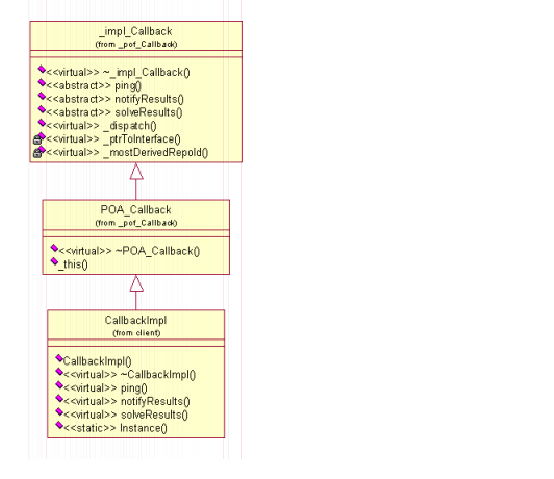
\includegraphics{./fig/CorbaClientClassDIagram}
  %\caption{UML Class diagram about Callback mecanism}
  %\label{fig:CorbaClientClassDIagram} 
  %\end{center}
  %\end{figure}

  Class constructor is private. It is accessed by a static class function
  \emph{CallbackImpl::instance} which returns a sole object instance. It
  creates object, initialises its class data and CORBA context, provides a
  client callback CORBA server on network.
  Client code must only give its CORBA reference when calling asynchronous
  function \emph{solveAsync}.s
  SeD server calls \emph{CORBA} \emph{solveResult} function with this
  reference to send results to client callback server.
  Combining  a call to \emph{diet\_initialise} and DIET file option
  \emph{useAsyncCall} automates client callback mecanism.
  A \emph{diet\_finalize} call unactivates callback server, destroys
  CallbackImpl object and Object Request Broker data.

  \paragraph{synchronizing data}
  Synchronising access on data is necessary because of:
  \begin{itemize}
  \item Threads can together retrieve results data.
  \item CORBA threads pool from client callback server read concurrently
  profil data structure.
  \item DIET API function \emph{diet\_wait*} stop caller thread until wait
  results data are arrived on client.
  \end{itemize}
  Classes from following UML diagram resume these drawbacks.

  %\begin{figure}[h]
  %\begin{center}
  %\centering
  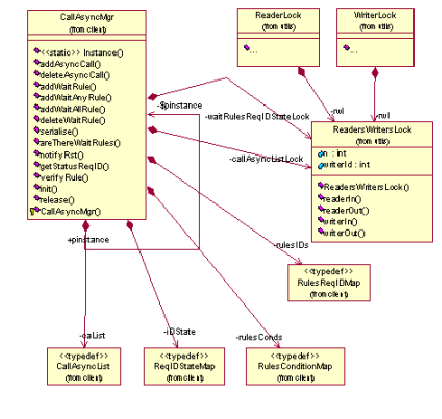
\includegraphics{./fig/CallBackSynchronisationClassDiagram2}
  %\caption{Diagramme UML class diagram about callbackImpl and GridRPC/DIET asynchronous functions}
  %\label{fig:CallBackSynchronisationClassDiagram2}
  %\end{center}
  %\end{figure}

  CallAsyncMgr manages synchronising mecanism on wait results. It is a \emph{thread-safe}
  singleton which locks access on share data and race condition code. A
  \emph{diet\_initialise}/\emph{diet\_finalise} call creates/destroys it. A
  Reader/Writer lock mecanism (exception-safe) manages syncronising between
  CORBA and DIET client threads.

  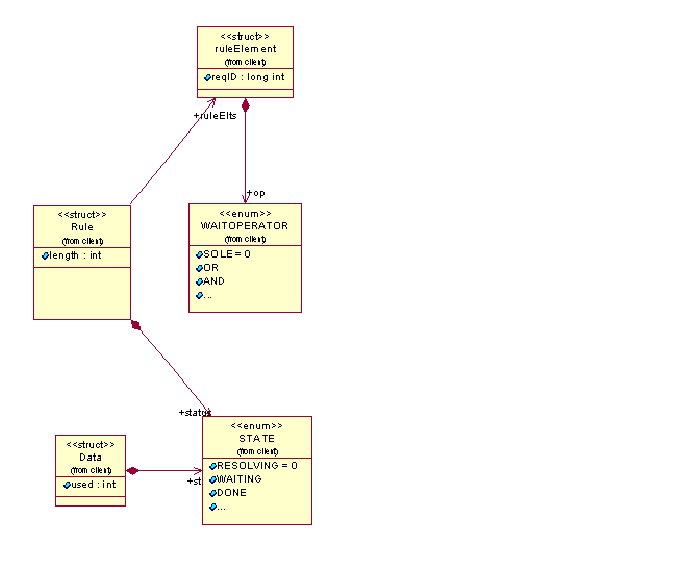
\includegraphics{./fig/WaitRulesClassDiagram}

  \emph{CallAsyncMgr} register/unregister asynchronous calls, their request
  identifiers and data by \emph{addAsyncCall}/ \emph{deleteAsynCall} methode.
  It stops client threads with addWait* methodes. These methodes have
  parameters which store conditions on retrieved results to unlock threads.
  A \emph{Rule} structure contains a set of three data (request identifier,logical operator, state).
  Two list of data pair (\emph{RulesConditionMap} and \emph{CallAsyncList}) map \emph{Rule} with a
  lock reference and request identifier with a DIET data
  profil. \emph{notifyRst} methode allows CORBA threads to announce results getting,
  update data in memory client space, unlock one or more waited threads.

  %\subsubsection{Synchronising and interworking}
  \paragraph{Synchronising and interworking}
  In following scenarios, an UML actor figures user client code with DIET/GridRPC API.

  \subparagraph{Asynchronous call on a SeD:}
  This first scenario shows a begining of an asynchronous solve.

  %\begin{figure}[h]
  \hspace{-0.9 in}
  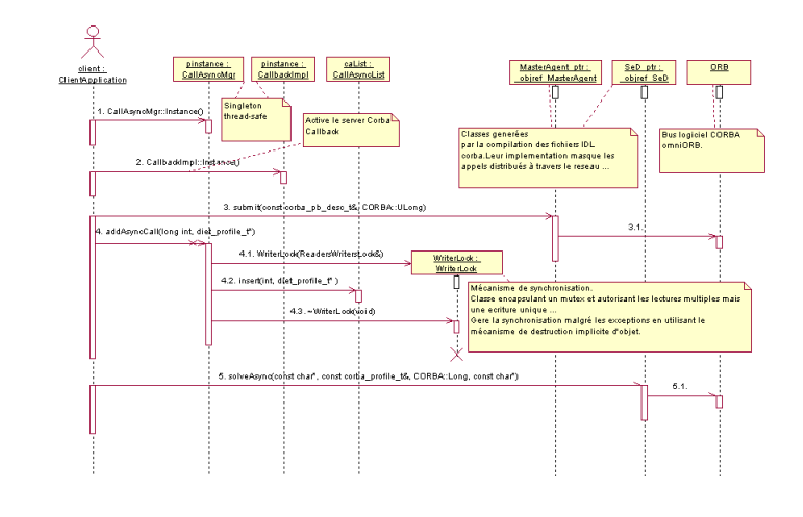
\includegraphics{./fig/CallAsyncSequenceDiagram}
  %\end{figure}

  After creating CallbackImpl and callAsyncMgrby a call to
  \emph{diet\_initialize}, client execute submit function specifying DIET
  problem. Then, \emph{addcallAsync} methode stores a sole request
  identifier and managed memory space and \emph{solveAsync} starts
  asynchronous solve.
  CallAsyncList is a C++ container \emph{list} from \emph{Standard Template Library}
  \emph{ORB} entity is a virtual object figuring CORBA services API like
  marshalling, network traffic and CORBA object binding.
  Client thread can wait for notify event about satisfied conditions or
  poll results states by frequently call to \emph{getStatusReqId} methode.

  \vspace{.9 in}

  \subparagraph{Thread Waiting for results and then continue:}
  Solve is started and client thread can wait for results.

  \hspace{-1 in}
  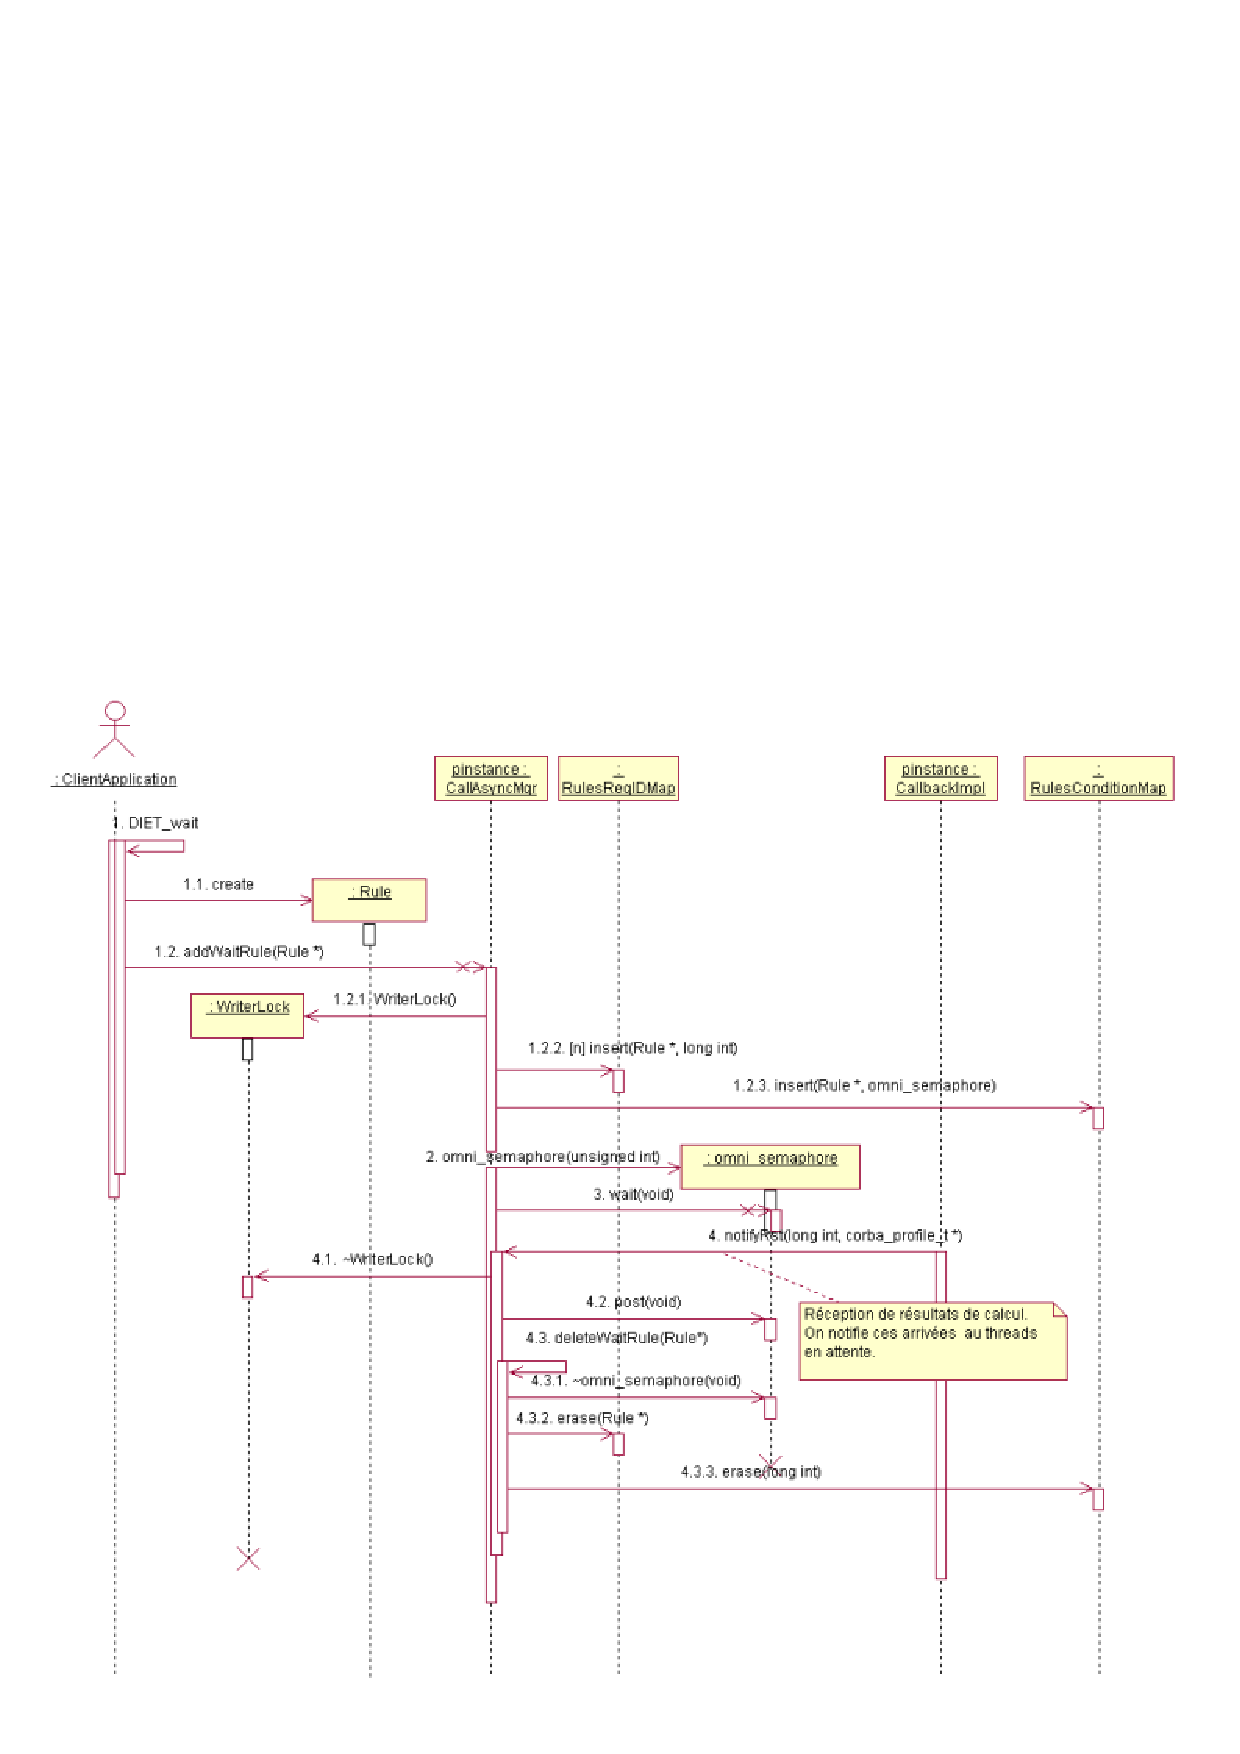
\includegraphics{./fig/CallAsyncWaitSequenceDiagram}

  Client code can use synchronising functions like \emph{diet\_wait*}
  in GridRPC/DIET API to wait for results. The following text describes
  this mecanism.

  After calculus starting, client creates a waiting Rule which specifies
  waiting conditions. Then it calls \emph{addWaitRule} methode which do :

  \begin{itemize}
  \item locks synvhronising mecanism.
  \item validates rule data (request identifier, etc).
  \item registers the rule.
  \item creates an \emph{omniORB}  semaphore, maps to the rule, registers it,
  unlocks synchonising mecanism (\emph{WriterLock}) and call its \emph{wait} methode.
  \item during call to \emph{notifyRst} methode by \emph{Callback} server
  (\emph{calbackImpl}), finds all rules whose conditions are verified
  and unlock their semaphores.
  \item frees memory linked to rule data and returns a \emph{STATE} enum
  which defines five state (RESOLVING, WAITING, DONE, CANCEL, ERROR). If
  a calculus is stopped during its executing process (with a call to deleteCallAsync for example),
  CANCEL is returned. If thread catches an error or an exception, ERROR is returned else DONE is returned.
  \end{itemize}


  \subparagraph{Getting results into callback server and notifying them to waiting threads :}
  This scenario figures notifying available results into client. It completes
  the previous algorythm about threads using client gridRPC API which is a
  part of DIET client library.

  \begin{center}
  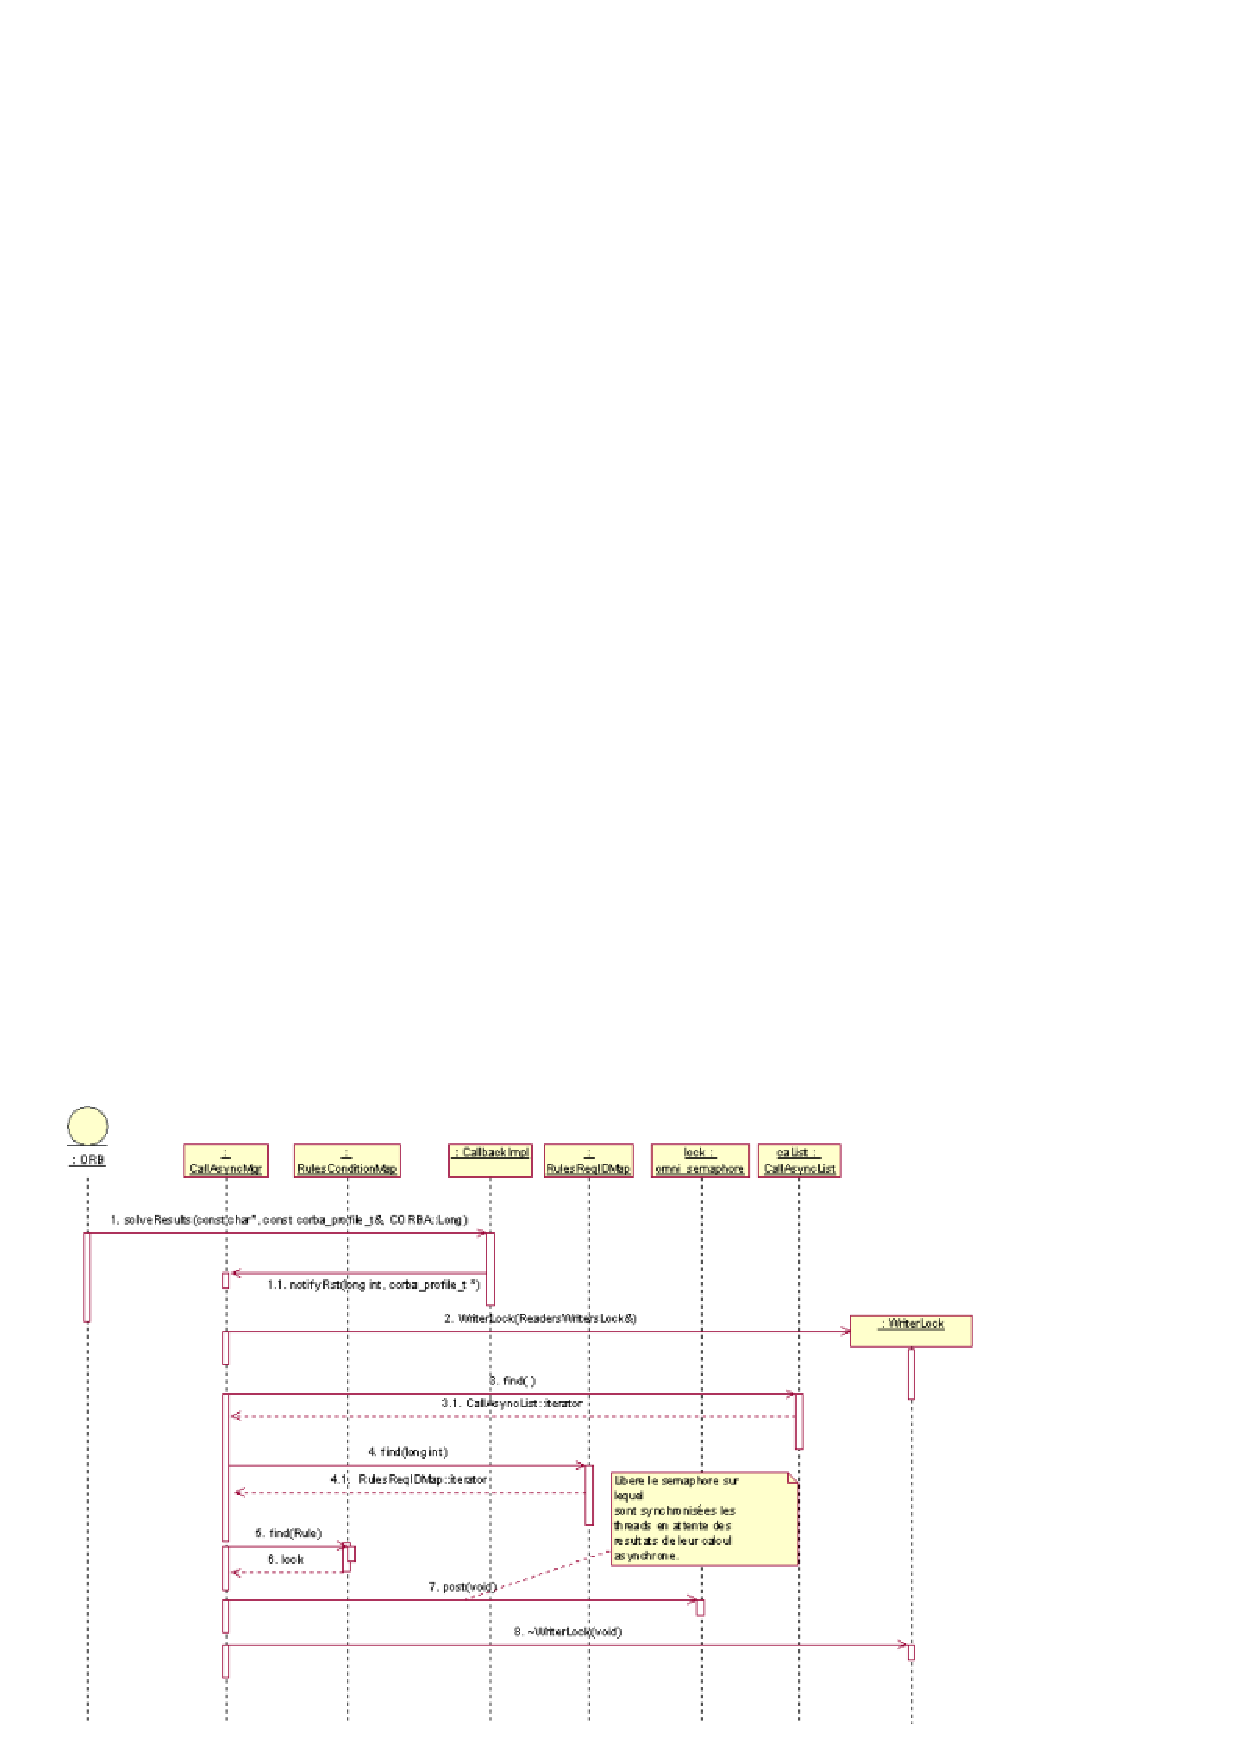
\includegraphics{./fig/CallbackSynchronisationSequenceDiagram}
  \end{center}

  \begin{itemize}
  \item SeD pushes results on client by a CORBA call to \emph{solveResults}.
  \item Callback server notifies available results by a call to \emph{notifyRst}.
  \item locks synchronising mecanism (\emph{WriterLock}).
  \item validates data and request identifier(\emph{find}).
  \item finds rules linked to retrieved results.
  \item verifies all rules waiting conditions.
  \item unlocks waiting threads linked to these rules.
  \item unlocks synchronising mecanism (\emph{~WriterLock}).
  \end{itemize}

  \subparagraph{Getting result state by an asynchronous function:}
  Unlike local synchronous call as \emph{addWait*}, client can get results
  state with \emph{getStatusReqId}. This call returns an enum type \emph{STATE}
  which defines five state (RESOLVING, WAITING, DONE, CANCEL, ERROR).
  \emph{CallAsyncMgr::addWait*} returns also this enum.
  RESOLVING announces that calculus goes on, WAITING that is not started,
  DONE that is finished and results are availabale, CANCEL that is stopped
  by user and ERROR that is stopped by an error or an exception.

  \begin{center}
  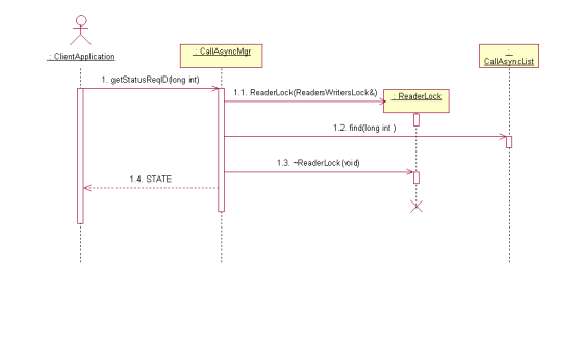
\includegraphics{./fig/CallAsyncProbeSequenceDiagram1}
  \end{center}

  \begin{itemize}
  \item call of \emph{CallAsyncMgr::getStatusReqId}.
  \item lock synchronising mecanism.
  \item verify calculus identity and validity.
  \item get state linked to calculus.
  \item unlock synchronising mecanism.
  \end{itemize}

  \noindent
  \fbox{\textbf{NB}} This algorythm is also used by \emph{diet\_probe} function
  into GridRPC API.

  \subparagraph{Managing memory in asynchronous request:}
  \emph{CallAsyncMgr::deleteAsyncCall} frees internal data linked to a
  calculus if it is finished, its results are available and no rule includes
  it into its waiting conditions.
  If others rules are linked to this result, their state are modified to
  CANCEL as well as calculus state linked. Then synchronising mecanisms
  are unlocks, threads goes on and \emph{CallAsyncMgr::addWait*} returns
  CANCEL state. Finally, memory is free.

  \begin{center}
  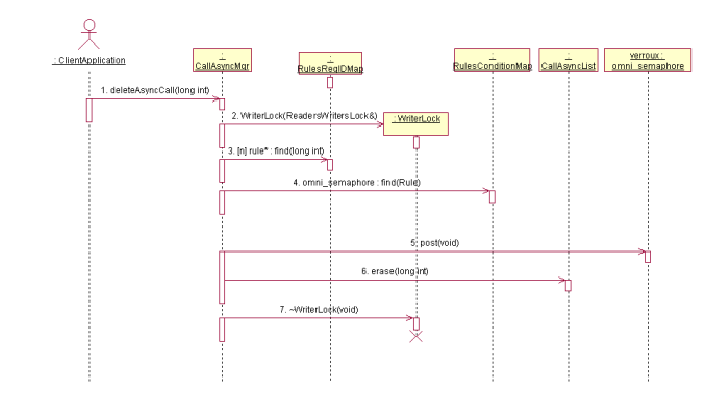
\includegraphics{./fig/DietCancelSequenceDiagram}
  \end{center}

  \begin{itemize}
  \item call of \emph{callAsyncMgr::deletecallAsync}.
  \item lock synchronising mecanism.
  \item verify request identifier.
  \item look for rules linked to request identifier,
  unlock synchronising items and fix rule state with CANCEl.
  \item free memory alocated to rule data and mutexes.
\item free data about request (request identifier, state, ...)
  \end{itemize}

  \noindent
  \fbox{\textbf{NB}} These algorythms only concern client processus. Next development steps
  will provide direct interactions to SeD server processus using persistence
  service.

  \section{\textsf{src/CORBA}}
  \label{s:CORBA}

  \subsection{\textsf{ORBMgr}}

  This module has been written to hide the ORB to the rest of the code. The idea
  is that every ORB-dependent operation might be performed through a unified API,
  described in \textsf{ORBMgr.hh}. Of course, DIET still supports only omniORB,
  but soon it should support TAO too.
  \\
  This module does not aim at unifying the APIs of the various thread libraries of
  such ORBs. As this should be a part of the DIET API, it should be processed in
  what \textsf{DIET\_mutex} could become.
  \\
  It has been decided to add to this module some of the usual OMG calls, so that
  it is easier to initialize, bind its name in the naming service, etc.


  \subsection{Data memory management}

  \fixme{Bruno - Help me please, if I have no time ...}


  \subsection{Convertors}

  \fixme{under construction ...}



  \section{\textsf{src/CORBA/idl}}
  \label{s:IDL}

  In this directory, all IDL interfaces have been gathered. They are organized as
  follows:
  \begin{description}
  \item {\sf common\_types.idl}: all (almost all) types used in all the
  communications of the platform.
  \item {\sf response.idl}: the structure of a response, with the sorted
  (scheduled) lists of servers.
  \item {$[$\textsf{Local$|$Master}$]$\textsf{Agent.idl}, \textsf{Callback.idl} and \textsf{SeD.idl}}: the interfaces of the CORBA objects of the hierarchy.
  \end{description}
  Note that the type \texttt{corba\_estimation\_t} should be declared in
  \textsf{response.idl}, since it is a part of a response. But this would
  introduce a crossed-dependency: \textsf{response.idl} includes \textsf{SeD.idl}
  because a response contains the references to the servers, and \textsf{SeD.idl}
  needs the \texttt{corba\_estimation\_t} to be declared for the method
  \textsf{checkContract}. So, to get rid of the crossed-dependency, the type is
  declared in \textsf{common\_types.idl}.
  \\

  Compiling the IDL interfaces is a bit more complex than for any C or C++ file.
  Automake has no mechanism to manage IDL files, except the
  \texttt{BUILT\_SOURCES} variable. This variable stores all the C++ files
  generated by the compilation of the IDL files\footnote{The names of these files
    depend from the IDL compiler, but most of the compilers let the user choose
      the nomenclature}. But we must still specify the dependencies of the built
      sources from the IDL files. This is the role of the file \textsf{idlRules.mk}.

      \textsf{idlRules.mk} is included in Makefile.am defining compiling and linking rules
      with idl generated stubs files ( with omniORB, xxSK.cc and xxDynSK.cc). It contains
      a list of idl files, rules, targets, list of cleaned files and fixes a python
      bug.

      %    \fixme{Christophe - Explain the \textsf{idlRules.mk} - its role in the
        %     compilation chain}


        \section{\textsf{src/examples}}
        \label{s:examples}

        This directory contains the examples distributed with DIET. Its compilation
        depends on the configure option \texttt{--enable-examples}, forced in
        maintainer, and disabled by default for users.

        There are five complete applications, providing a server and one or several
        clients able to use the service(s) offered by the server. Two of them require
        special libraries to be installed on the machine, which are more or less
        detected at configuration time, but there is still much work to do for
        the automatic detection.

        \subsubsection{file\_transfer}

        This example was aimed to show how to manipulate the \texttt{DIET\_FILE} type.
        The client sends two files to the server. The second file is re-transfered
        without any change, since it is an INOUT, and its size is returned as an OUT.
        It shows the drawback of the file management: it is impossible for the user to
        gain control over the path of the received files.

        \subsubsection{scalars}

        This example was aimed to show how to manipulate the \texttt{DIET\_SCALAR} type,
        and the various modes of passing arguments. It shows the problems of the
        management of the base types in DIET: the length of the given data is not
        checked, and the correspondance with the CORBA types is still to be perfected.
        Actually, the length of the base types has been defined according to the
        NetSolve types, but it would have been more clever to accord them with the CORBA
        types.

        \subsubsection{dmat\_manips}

        The server offers an interface to some basic double matrix manipulations:
        transpose, product and sum. To make the clients of the examples
        \texttt{dmat\_manips}, \texttt{BLAS} and \texttt{ScaLAPACK} interchangeable for
        some problems, the profiles for services \texttt{MatPROD}, \texttt{SqMatSUM}
        (square matrix sum) and \texttt{SqMatSUM\_opt} (``optimized'' because the second
                                                        operand is INOUT) are the same. Thus, for a demo, a matrix product can be
        invoked by a client, and executed either on a server having the BLAS library
        installed, or a server performing only a basic matrix product (usually far much
            slower), according to the FAST estimation.
        \\

        Although there are many examples of convertors in this and other examples, the
        service \texttt{T}, the first written, was designed to give an example of
        remanipulation of the arguments. When FAST 0.4 has been integrated into DIET,
        all other services had to include convertors.

        Another step has been done for FAST 0.8. The convertors had to be rewritten
        since the matrix type has been suppressed from the FAST API (with all high-level
            descriptions of the problems) The idea is to create a profile, through the
        convertor, that has got only the arguments declared in the LDAP base (which can
            be extracted from the others), followed by the arguments that the computation
        needs. It was not possible to do that with FAST 0.4 because it was not designed
        to ignore unknown arguments. That is why we are forced to include
        \textsf{DIET\_config.h}, to get the version of FAST.
        \\

        %\fixme{Christophe - Please explain the asynchronous clients.}
        \texttt{dmat\_manips} contains also client samples about asynchronous call API. All
        use \texttt{diet\_call\_async} to start solve on SeD but each example shows
        a distinct function of asynchronous DIET API to get results. Like synchronous
        client, you can ask solving a SUM/PROD/T operation on SeD. Besides, they are
        \texttt{multithreaded}. You can specify thread number of a pool and solve number. Each
        thread cucurently sends data to SeD(s) and gets results according to its used
        \texttt{diet\_wait\/probe\_*} function.
        \texttt{parallelclient.cc} retrieves results by a simple \texttt{diet\_wait} function
        and \texttt{parallelclient2.cc} by a peridical \texttt{diet\_probe} call.
        \texttt{parallelclient3.cc} and \texttt{parallelclient3.cc} are examples about
        respectivly \texttt{diet\_wait\_and} and \texttt{diet\_wait\_or}. Executing
        one of these examples prints traces about calculus parameters, synchronizing
        mecanisms on threads and results.

        \subsubsection{BLAS}

        To compile the BLAS server, you will need the BLAS library installed. For
        developers using a Linux Debian, there is a package, and everything has been
        performed for the configure to take such a package into account: just use the
        \texttt{--enable-BLAS} option, and it should be automagically detected. For
  other installations, it might be necessary to use all the arguments defined by
the ACI\_PACKAGE macros (\texttt{--with-BLAS=}, ...)

  So far, this server provides the \texttt{dgemm} service and all its derivations:
  \texttt{MatPROD}, \texttt{SqMatSUM}, \texttt{SqMatSUM\_opt} and
  \texttt{MatScalMult}. Convertors are used to convert the profiles of the
  problems to the one of the pdgemm service, so that only one solve function has
  to be implemented. But this server is destined to be an interface to all the
  functions of the BLAS library.
  \\

  We have the same problem of compatibility with FAST 0.4 and FAST 0.8 in the BLAS
  server as in the dmat\_manips example. Actually, this server only supports
  FAST 0.4, since the modifications to get low-level profiles for FAST 0.8 have not
  been done yet. But these modifications are quite similar to the ones of the
  dmat\_manips server, and they will be easy to add.

  \subsubsection{ScaLAPACK}

  It is very difficult to detect all the libraries necessary to compile a program
  calling the \texttt{pdgemm} function. Nothing has been done actually for it in
  the \texttt{configure.ac}, because not only the LAPACK library should be found,
  but also an MPI implementation, etc. Nevertheless it is still possible to
  compile the server of this example if the user knows exactly all the paths for
  these libraries, or the extra arguments to compile with them (through
      \texttt{--with-ScaLAPACK-extra}), thanks to the \texttt{ACI\_PACKAGE} macros
  from M. Quinson.

  So far, this server provides the \texttt{pdgemm} service and all its
  derivations: \texttt{dgemm}, \texttt{MatPROD}, \texttt{SqMatSUM},
  \texttt{SqMatSUM\_opt} and \texttt{MatScalMult}. Convertors are used to convert
  the profiles of the problems to the one of the pdgemm service, so that only one
  solve function has to be implemented. But this server is destined to be an
  interface to all the functions of the ScaLAPACK library.

  The implementation of this SeD is complex. It is launched on the node 0 of an
  MPI grid. When the client submits a problem, it asks for a number of nodes to
  execute the computation. Then, the node 0 creates a subgrid of the available
  nodes and launches the computation on this new grid. Of course, depending on the
  number of nodes required by the client, and the number of nodes still available
  in the initial grid, it is possible that the computation returns with an error
  code, or that the same node is used for several processes.
  \\

  The support for FAST is quite difficult to add, since the server is supposed to
  be parallel. Maybe we should wait for the FAST/Freddy integration to be
  complete.



  \section{\textsf{src/SeD}}
  \label{s:SeD}

  This directory contains the implementations of
  \begin{itemize}
  \item the DIET server API,
  \item the IDL interface of the SeD.
  \end{itemize}
  \

  The functions of the API are easy to understand, as far as the User's Manual is
  well understood. They use a global static variable \texttt{SRVT}, and its
  manipulation is not thread-safe, since it would have no sense to launch two SeDs
  with the same service table in two different threads.
  \\

  There is nothing else important to explain in the implementation of the IDL
  interface but the \texttt{solve} methods. These methods run on the same
  scheme, except that \texttt{solveAsync} is \textit{oneway}, ie. asynchronous,
  and thus it has to send explicitly the results, through a callback mechanism, at
  the end of the computation.

  %\fixme{Christophe - the callback mechanism might require some more explanations}
  In case of asynchronous call, i.e solve\_async call, client specifies a request
  identifier and a CORBA reference defining its Callback client server (IP/Port).
  And thus, at the end of the solve, the \texttt{solveAsync} function call \texttt{notifyRst}
  of client callback server with diet profile and request ID parameters. Client manages
  callback threads, results and notifying news through its asynchronous API.
  After this calling, SeD thread free memory.

  Both methods have to ``unmarshall'' the arguments, ie. to convert them into DIET
  data that the programmer of the server can manipulate. Then they invoke the
  solve function through the pointer given by this programmer, and reconvert
  (marshall) the OUT data into CORBA data to be sent back on the client. Thus the
  computation is performed inner a CORBA thread, created at the remote invokation
  of the method.

  To perform the computation in a separate process, we will be forced to dump the
  arguments into files ... It is still to be done.


  \section{\textsf{src/utils}}
  \label{s:utils}

  This directory gathers all tools and utils that are used by more than one
  entity of DIET.

  \fixme{under construction ...}

  \subsection{\textsf{Counter}}

  The \texttt{Counter} class implements a thread safe counter. This counter
  accepts only 32 bits positive value. This class must be used each time a
  counter is shared by several threads. Read the doxygen documentation for more
  informations about how-to use it.

  \subsection{\textsf{ms\_function}}

  Several calls to \texttt{strdup()}, \texttt{CORBA::string\_dup()},
  \texttt{malloc()} and \texttt{stralloc()} are made inside the DIET code. The
  problem is : each of these functions can return the \texttt{NULL} value. The
  use of an allocated memory without testing the \texttt{NULL} value will
  probably result to a segmentation fault if there was not enough memory. This
  is why the \textsf{ms\_function} file describes some functions which allocate
  the memory and test if the \texttt{NULL} value is returned. If it is the case,
  a \texttt{bad\_alloc} exception is thrown, if not the functions behave like the
  standard ones. Read the doxygen documentation for more informations about
  how-to use them.

  \subsection{\textsf{ts\_container}}

  The C++ Standard Library gives access to several containers. A map, a vector, a
  list and a set templates are defined by the C++ Standard. The only problem with
  them is that there are not thread safe. If two threads alter a container at the
  same time, a crash is on the way. Therefore a critical section access mechanism
  must be implemented to avoid it. It is easy to forgot to lock the access to a
  list before using it. This is why the \texttt{ts\_container} exists (the
      \texttt{ts} is for Thread Safe). They managed the access to there critical
  section by themselves. All the list and set which are shared by several threads
  must be implemented with a \texttt{ts\_container} to avoid a simultaneous
  access to it. Read carefully the doxygen documentation to know which one to use
  and how-to use it.

\section{\textsf{cmake}}
\label{s:cmake}

This directory gathers the cmake related scripts that cmake authorizes to
be deported here.
